\clearpage

\appendix




\section{Downstream Task Details}

Table~\ref{tbl:paramter} shows the hyperparameters that we use for finetuning on the downstream vision-language tasks.
All tasks uses AdamW optimizer with a weight decay of 0.05 and a cosine learning rate schedule.
We use an image resolution of $384\times384$,
except for VQA where we follow~\citet{simvlm} and use $480\times480$ images.
Next we delineate the dataset details.

\noindent\textbf{Image-Text Retrieval.}
We use the Karpathy split~\cite{karpathy} for both COCO and Flickr30K.
COCO contains 113/5k/5k images for train/validation/test,
and Flickr30K contains 29k/1k/1k images for train/validation/test.

\noindent\textbf{Image Captioning.}
We finetune on COCO's Karpathy train split,
and evaluate on COCO's Karpathy test split and NoCaps validation split.
During inference,
we use beam search with a beam size of 3,
and set the maximum generation length as 20.

\noindent\textbf{VQA.}
We experiment with the VQA2.0 dataset~\cite{VQA2}, which contains 83k/41k/81k images for training/validation/test.
Following~\citet{ALBEF},
we use both training and validation splits for training, and include additional training samples from Visual Genome.
During inference on VQA,
we use the decoder to rank the 3,128 candidate answers~\cite{ALBEF,bilinear}.

\noindent\textbf{NLVR$^2$.}
We conduct experiment on the official split~\cite{NLVR}.

\noindent\textbf{VisDial.}
We finetune on the training split of VisDial v1.0 and evaluate on its validation set.


\begin{table}[!h]
   % \small
	\centering	
    %\setlength\tabcolsep{3pt}
	%\resizebox{1\columnwidth}{!}{%
	\begin{tabular}	{l   |  c  c  c }
		\toprule	 	
	 Task & init LR (ViT-L) & batch size & \#epoch \\
	 \midrule
	 Retrieval & $1e^{-5}$ ($5e^{-6}$) & 256 & 6  \\
	 Captioning & $1e^{-5}$ ($2e^{-6}$) & 256 & 5 \\
	 VQA & $2e^{-5}$ & 256 & 10 \\
	 NLVR$^2$ & $3e^{-5}$ & 256 & 15 \\
	 VisDial & $2e^{-5}$ & 240 & 20 \\ 		
		
% 	 \multirow{2}{*}{Task} & \multicolumn{3}{c|}{\name$_\mathrm{base}$} & \multicolumn{3}{c}{\name$_\mathrm{large}$} \\
% 	 & init LR & batch size & \#epoch & init LR & batch size & \#epoch\\
% 	 \midrule
% 	 Retrieval & $1e^{-5}$ & 256 & 6 & & & \\
% 	 Captioning & $1e^{-5}$ & 256 & 5 & & & \\
% 	 VQA & $2e^{-5}$ & 256 & 10 & & & \\
% 	 NLVR$^2$ & $3e^{-5}$ & 256 & 15 & & & \\
% 	 VisDial & $2e^{-5}$ & 240 & 20 & & &\\ 
		\bottomrule
	\end{tabular}
 	%}
 	 \vspace{-1ex}	
	\caption
	{
	\small	
		Finetuning hyperparameters for downstream tasks.
	}
	\label{tbl:paramter}
 \vspace{-2ex}	
\end{table}		


\begin{figure*}[!b]
\centering
  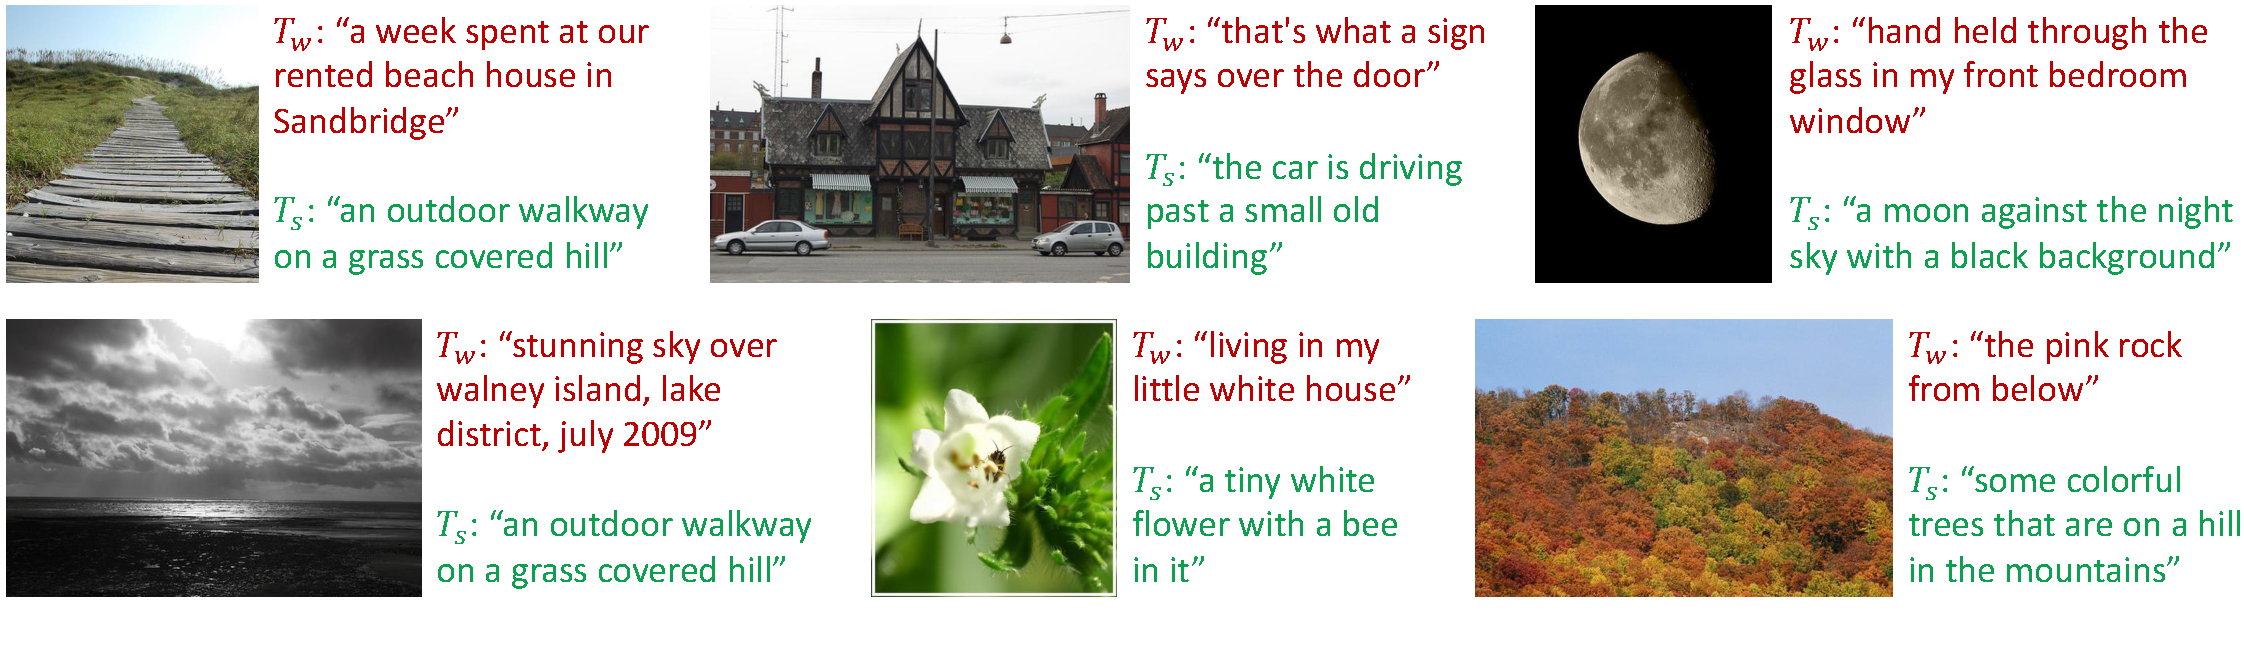
\includegraphics[width=\textwidth]{imgs/more_examples.pdf}
\vspace{-6ex}
\caption{Examples of the web text $T_w$ and the synthetic text $T_s$. {\color{ForestGreen}Green} texts are accepted by the filter,
whereas {\color{BrickRed}red} texts are rejected.
}
\label{fig:more_example}
\end{figure*}

\vspace{-0.5ex}
\section{Additional Examples of Synthetic Captions}
In Figure~\ref{fig:more_example},
we show additional examples of images and texts where the web captions are filtered out, and the synthetic captions are kept as clean training samples.



\section{Pre-training Dataset Details}

Table~\ref{tbl:pretrain_data} shows the statistics of the pre-training datasets.
\begin{table}[!h]
	\small
	\centering	
	\setlength\tabcolsep{4pt}
	\resizebox{\columnwidth}{!}{%
		\begin{tabular}	{l   |  c c c c c c}
			\toprule
			  & COCO & VG  & SBU & CC3M & CC12M & LAION \\
			\midrule
			\# image  & 113K & 100K & 860K & 3M & 10M & 115M\\
			\# text & 567K & 769K & 860K & 3M & 10M & 115M\\
			\bottomrule
		\end{tabular}
	}
	\vspace{-2ex}	
	\caption
	{
		\small	
		Statistics of the pre-training datasets.
	}
	\label{tbl:pretrain_data}
	\vspace{-1ex}	
\end{table}